%*********************************************************
% Federal University of Santa Catarina (UFSC)
% 
% Author: 				Gabriel Mariano Marcelino
% 
% Created on: 			13/12/2017
% Last modification: 	14/12/2017
%*********************************************************

\documentclass[12pt]{book}
\usepackage[a4paper,left=2.5cm,right=2.5cm,top=2.5cm,bottom=2.5cm]{geometry}
\usepackage[T1]{fontenc}  
\usepackage[utf8]{inputenc} 
\usepackage[english]{babel}
\usepackage{ae}
\usepackage{graphicx}
\usepackage[hidelinks]{hyperref}
\usepackage{fancyhdr}
\usepackage{subfigure}
\usepackage{nomencl}
\usepackage{float}
\usepackage{titlesec}
\usepackage{booktabs}
\usepackage{emptypage}
\usepackage{lettrine}

\title{Telemetry, Tracking and Command Module of the FloripaSat Project}
\author{Gabriel Mariano Marcelino}
\date{13/12/2017}

% File metadata
\hypersetup
{
    pdfauthor	={Gabriel Mariano Marcelino},
    pdfsubject	={Telemetry, Tracking and Command Module Documentation},
    pdftitle	={Telemetry, Tracking and Command Module of the FloripaSat Project},
    pdfkeywords	={Cubesats, TTCs, Telecomunications}
}

% URLs font style
\urlstyle{same}

% First chapter page style
\titleformat{\chapter}[display]
	{\bfseries\Large}
	{\filright\MakeUppercase{\chaptertitlename} \Large\thechapter}
	{1ex}
	{\titlerule\vspace{1ex}\filleft}
	[\vspace{1ex}\titlerule]

% Header style
\pagestyle{fancy}
\fancyhf{}
\fancyhead[RO]{Telemetry, Tracking and Command Module}
\fancyhead[LE]{\nouppercase{\leftmark}}
\fancyfoot[RO]{\thepage}
\fancyfoot[LE]{\thepage}
\renewcommand{\footrulewidth}{0.5pt} 

% List of abbreviations
\makenomenclature
\setlength\nomlabelwidth{1.5cm}

% Bibliography style
\bibliographystyle{unsrt}

\begin{document}

\begin{titlepage}

%****************************************************
%****************************************************
%-- TITLE PAGE --------------------------------------
%****************************************************
%****************************************************
\thispagestyle{empty}

\begin{flushleft}
FLORIPASAT - TTC-DOC - REV1
\end{flushleft}

\begin{figure}[!ht]
	\begin{flushleft}
		
\includegraphics[width=5cm]{figures/floripasat.png}
	\end{flushleft}
\end{figure}

\begin{flushleft}
\Huge{\textbf{Telemetry, Tracking and Command Module of the FloripaSat Project}}
\rule[0pt]{\textwidth}{5pt}
\end{flushleft}

\vspace{0.2cm}

\begin{flushleft}
\textit{Module Documentation} \\
\textit{GSE, Federal University of Santa Catarina, Florianópolis - Brazil}
\end{flushleft}

\vfill
\vfill

\begin{flushright}
December 2017
\end{flushright}

\pagenumbering{roman}
\setcounter{page}{1}

\end{titlepage}

\cleardoublepage

%****************************************************
%****************************************************
%-- AUTHOR PAGE -------------------------------------
%****************************************************
%****************************************************

\thispagestyle{empty}

\begin{center}

\textbf{FloripaSat Project, Telemetry, Tracking and Command Module Documentation}

\textit{December, 2017}

\vspace{1cm}

\textbf{Project Manager:}

Eduardo Augusto Bezerra

\vspace{1cm}

\textbf{Author:}

Gabriel Mariano Marcelino

\vspace{1cm}

\textbf{Contributing Authors:}

Anselmo Luis da Silva Junior \\
Marcelo Daniel Berejuck \\
Sara Vega Martinez \\

\vspace{1cm}

\textbf{Layout:}

Gabriel Mariano Marcelino

\end{center}

\vspace{8cm}

\begin{figure}[!h]
%\begin{wrapfigure}{l}{0.25\textwidth}
	\begin{center}
		\includegraphics[width=0.25\textwidth]{figures/by-sa.eps}
	\end{center}
\end{figure}
%\end{wrapfigure}

\textcircled c 2017 by Federal University of Santa Catarina. Telemetry, Tracking and Command Module of the FloripaSat Project. This work is licensed under the Creative Commons Attribution-ShareAlike 4.0 International License. To view a copy of this license, visit http://creativecommons.org/licenses/by-sa/4.0/.

%****************************************************
%****************************************************
%-- ABSTRACT ----------------------------------------
%****************************************************
%****************************************************

\chapter*{Abstract}

This document...

\smallskip
\noindent \textbf{Keywords:} Cubesats. Embedded systems. Telecomunications.

%****************************************************
%****************************************************
%-- TABLE OF CONTENTS -------------------------------
%****************************************************
%****************************************************
\tableofcontents

%****************************************************
%****************************************************
%-- LIST OF FIGURES ---------------------------------
%****************************************************
%****************************************************

\listoffigures
\addcontentsline{toc}{chapter}{List of Figures}

%****************************************************
%****************************************************
%-- LIST OF TABLES ----------------------------------
%****************************************************
%****************************************************

\listoftables
\addcontentsline{toc}{chapter}{Lista of Tables}

%****************************************************
%****************************************************
%-- NOMENCLATURE ---------------------------
%****************************************************
%****************************************************

\printnomenclature
\addcontentsline{toc}{chapter}{Nomenclature}

%****************************************************
%****************************************************
%-- INTRODUCTION ------------------------------------
%****************************************************
%****************************************************

\chapter{Introduction}

\pagenumbering{arabic}

\lettrine{I}{ntroduction}...

\nomenclature{\textbf{TTC}}{Telemetry, Tracking and Command.}
\nomenclature{\textbf{PCB}}{Printed Circuit Board.}
\nomenclature{\textbf{USB}}{Universal Serial Bus.}

\cite{site}.

\section{Module Requirements}

%****************************************************
%****************************************************
%-- HARDWARE ----------------------------------------
%****************************************************
%****************************************************

\chapter{Hardware}

\lettrine{T}{he} TTC board is composed by the following main components:

\begin{itemize}
	\item MSP430F6659, as the beacon microcontroller.
	\item RF4463F30, as the radio module for the beacon and the telemetry link.
\end{itemize}

In the figure \ref{fig:ttc-board}, ...

\begin{figure}[!h]
	\begin{center}
		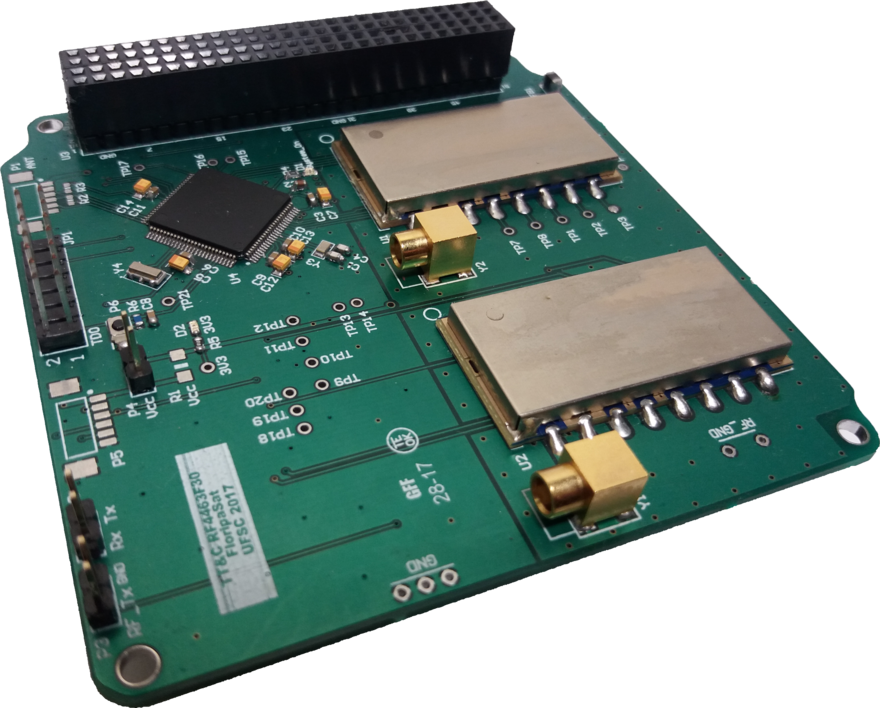
\includegraphics[width=0.75\textwidth]{figures/ttc_board.png}
		\caption{TTC PCB.}
		\label{fig:ttc-board}
	\end{center}
\end{figure}

\section{General Diagram}

In the figure \ref{fig:hardware-diagram}, a general hardware diagram can be seen.

\begin{figure}[!h]
	\begin{center}
		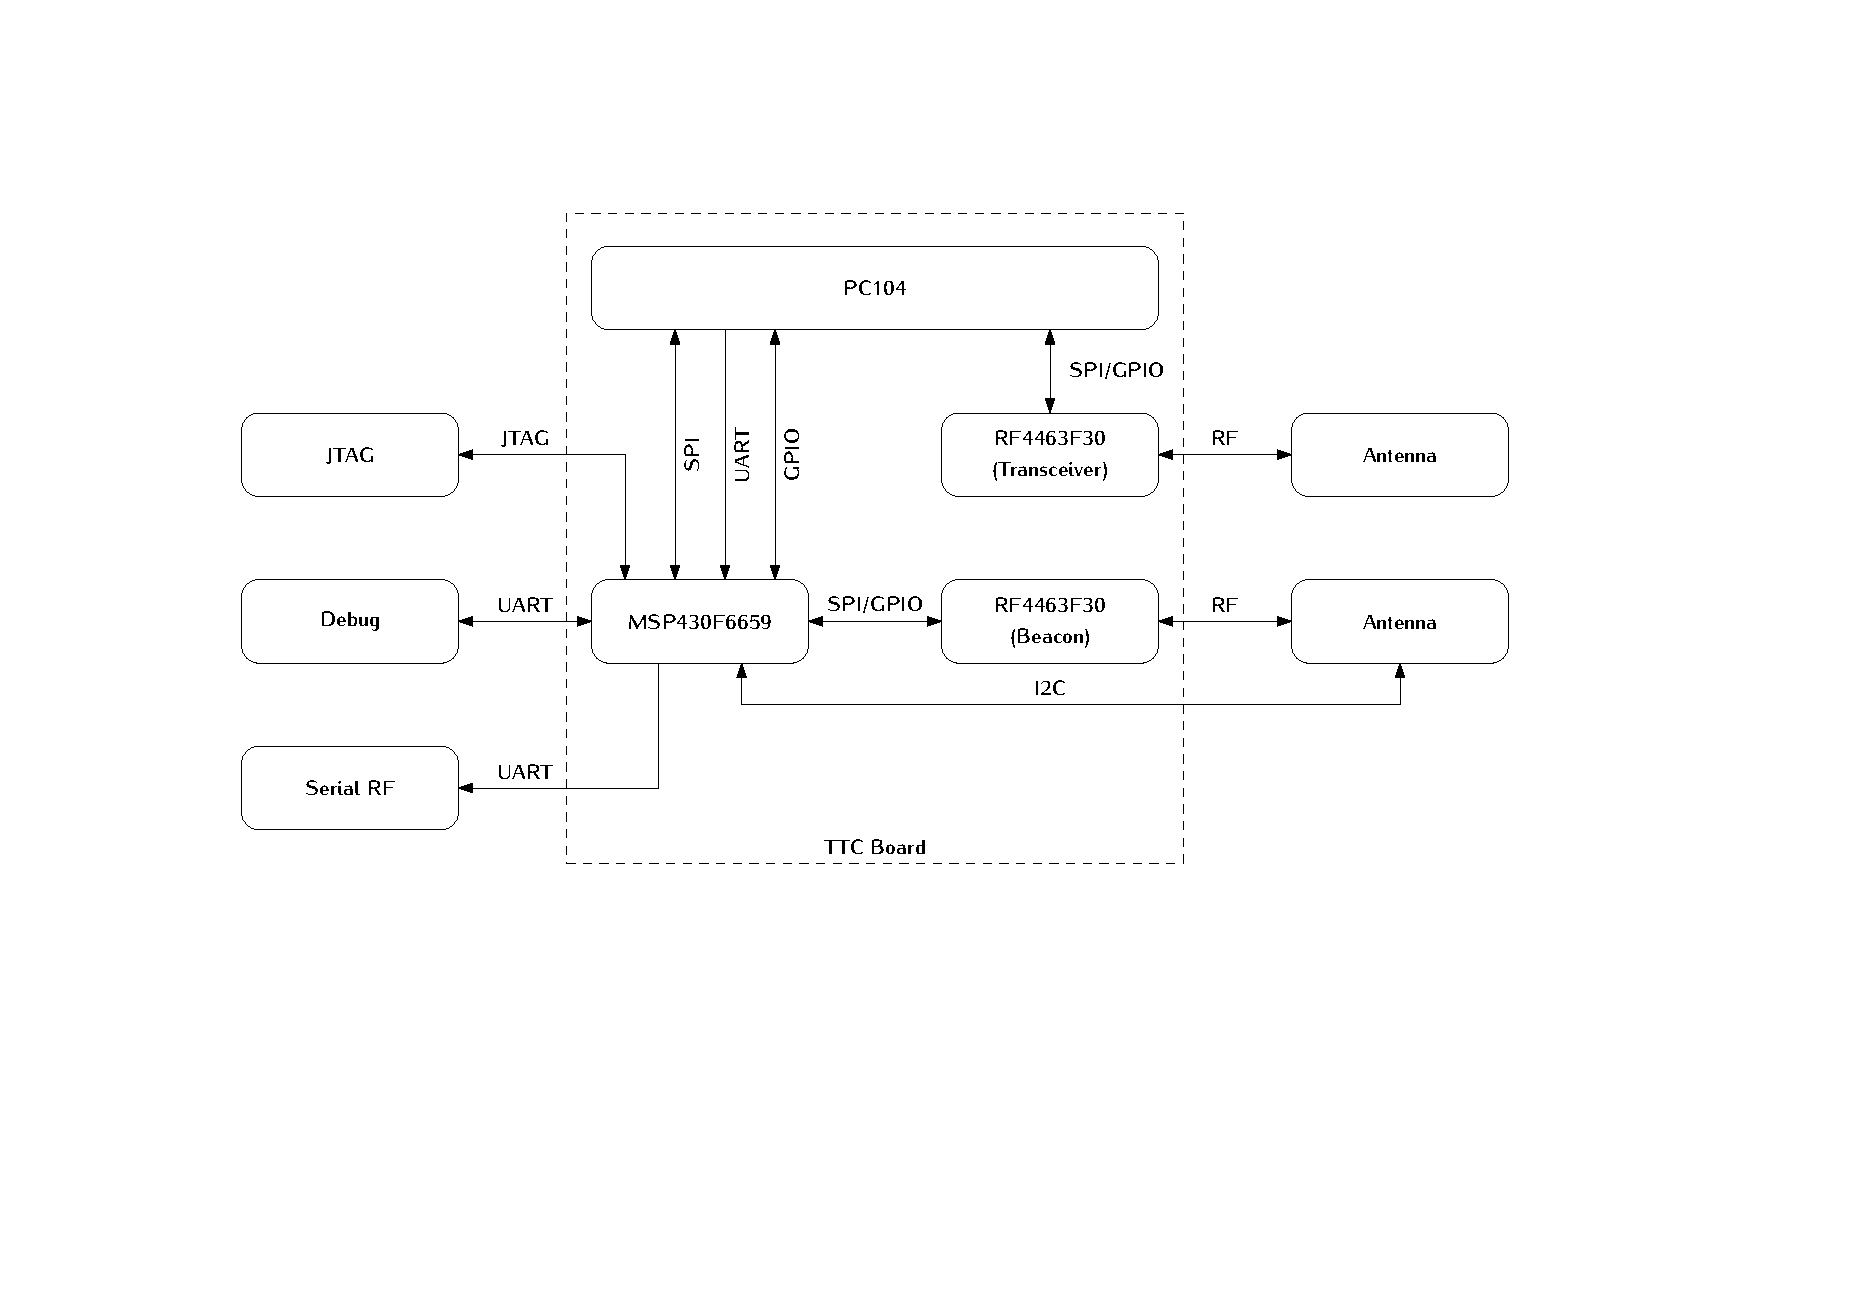
\includegraphics[width=\textwidth]{figures/hardware_diagram.pdf}
		\caption{Hardware diagram of the TTC module.}
		\label{fig:hardware-diagram}
	\end{center}
\end{figure}

\section{Main Components}

M...

\subsection{Microcontroller}

The beacon microcontroller is the MSP430F6659IPZR \cite{msp430f6659}. Its main characteristics can be found in the table \ref{tab:msp430f6659-info}.

\nomenclature{\textbf{CPU}}{Central Processing Unit.}
\nomenclature{\textbf{RAM}}{Random Access Memory.}
\nomenclature{\textbf{GPIO}}{General Purpose Input/Output.}
\nomenclature{\textbf{I$^{2}$C}}{Inter-Integrated Circuit.}
\nomenclature{\textbf{SPI}}{Serial Peripheral Interface.}
\nomenclature{\textbf{UART}}{Universal Asynchronous Receiver/Transmitter.}
\nomenclature{\textbf{DMA}}{Direct Memory Access.}
\nomenclature{\textbf{ADC}}{Analog-To-Digital Converter.}
\nomenclature{\textbf{BSL}}{Bootstrap Loader.}

\begin{table}[!h]
	\begin{center}
		\begin{tabular}{lc}
			\toprule[1.5pt]
			\textit{Characteristic} & \textit{Value} \\
			\midrule
			CPU & MSP430 \\
			Frequency & Up to 20 MHz \\
			Non-volatile memory & 512 kB \\
			RAM & 66 kB \\
			GPIO pins & 74 \\
			I$^{2}$C & 3 \\
			SPI & 6 \\
			UART & 3 \\
			DMA & 6 \\
			ADC & ADC12-12ch \\
			Comparators & 12 inputs \\
			Timers - 16-bit & 4 \\
			Multiplier & $32 \times 32$ \\
			BSL & USB \\
			Min $V_{cc}$ & 1,8 V \\
			Max $V_{cc}$ & 3,6 V \\
			Active Power & $360\ \mu A/MHz$ \\
			Standby Power (LMP3) & $2,6\ \mu A$ \\
			Wakeup Time & $3\ \mu s$ \\
			Operating Temperature Range & -40 to 80 $^{\circ}C$ \\
			\bottomrule[1.5pt]
		\end{tabular}
		\caption{MSP430F6659 features.}
		\label{tab:msp430f6659-info}
	\end{center}
\end{table}

\subsection{Radio Modules}

The NiceRF RF4463F30 \cite{rf4463f30} is a transceiver module based on the Silicon Labs Si4463 \cite{si4463} radio. This module also contains a PA module to increase the output power up to 31 dBm.

\subsubsection{Si4463}

\begin{table}[!h]
	\begin{center}
		\begin{tabular}{lcc}
			\toprule[1.5pt]
			\textit{Characteristic} & \textit{Value} & \textit{Unit} \\
			\midrule
			Frequency range & 119-1050 & MHz \\
			Receiver sensitivity & -126 & dBm \\
			Modulation & (G)FSK, 4(G)FSK, (G)MSK and OOK & - \\
			Max. output power & +20 & dBm \\
			PA support & +27 to 30 & dBm \\
			Ultra low current powerdown modes & 30 (shutdown), 50 (standby) & nA \\
			Data rate & 100 bps to 1 Mbps & - \\
			Power supply & 1,8 to 3,6 & V \\
			TX and RX FIFOs & 64 bytes for each or 129 bytes shared & - \\
			\bottomrule[1.5pt]
		\end{tabular}
		\caption{Si4463 features.}
		\label{tab:si4463-info}
	\end{center}
\end{table}

\section{External Connections}



\subsection{PCI104 Pins}



%****************************************************
%****************************************************
%-- SOFTWARE ----------------------------------------
%****************************************************
%****************************************************

\chapter{Software}

\lettrine{S}{oftware}...

%****************************************************
%****************************************************
%-- TESTS -------------------------------------------
%****************************************************
%****************************************************

\chapter{Tests}

\lettrine{T}{his}...

\section{RF Signal Power}

P...

%****************************************************
%****************************************************
%-- CONCLUSION --------------------------------------
%****************************************************
%****************************************************

\chapter{Conclusion} \label{ch:conclusion}

\lettrine{C}{onclusion}...

%****************************************************
%****************************************************
%-- REFERENCES --------------------------------------
%****************************************************
%****************************************************

\bibliography{references/site}
\addcontentsline{toc}{chapter}{Bibliography}

\end{document}
